\section{Preliminary Results}

\subsection{Quantification of TTX}

Table~\ref{tab:ttx} summarizes the reslts of TTX estimation using CIEIA.

\begin{small}\begin{longtable}[c]{lllllllll}
    % Caption and label
    \caption{Estimation of TTX concentration per specimen using CIEIA. Male individuals are identified by collection year (15), location (LW for Lake in the Woods and SC for Soup Creek), and number (7 or 8). \label{tab:ttx}} \\
    % Fist head
    \hline
    \hline
    \textbf{Spec.} & \textbf{SL} & \textbf{Skin} & \textbf{Mass} & \textbf{TTX} & \textbf{Final conc.} & \textbf{Whole newt} \\
     & \textbf{(cm)} & \textbf{(cm$^{2}$)} & \textbf{(g)} & \textbf{(ng/cm$^{2}$)} & \textbf{(ng/mL)} & \textbf{toxicity (mg)} \\
    \hline
    \endfirsthead
    % Last head
    \multicolumn{7}{c}{Continuation of Table \ref{tab:ttx}}\\
    \hline
    \textbf{Spec.} & \textbf{SL} & \textbf{Skin} & \textbf{Mass} & \textbf{TTX} & \textbf{Final conc.} & \textbf{Whole newt} \\
     & \textbf{(cm)} & \textbf{(cm$^{2}$)} & \textbf{(g)} & \textbf{(ng/cm$^{2}$)} & \textbf{(ng/mL)} & \textbf{toxicity (mg)} \\
    \hline
    \endhead
    % Contents
    15LW7 & 70 & 53.22 & 12.2 & 6.2673 & 0.443 & 0.000173 \\
    15LW8 & 70 & 66.41 & 16.6 & -5.7408 & -0.406 & -0.000198 \\
    15SC7 & 80 & 66.99 & 16.8 & 30098.4759 & 2127.101 & 1.046660 \\
    15SC8 & 75 & 65.55 & 16.3 & 35665.6123 & 2520.538 & 1.213594 \\
    \hline
\end{longtable}\end{small}

\subsection{Assembly statistics}

De novo transcriptome assemble for each biological replicate have 28-44\% complete, 8-14\% duplicate, 13-15\% fragmented and 41-55\% missing genes of 3,093 genes in the vertebrate genome dataset from BUSCO. The transcriptome build as reference including sequence reads from all biological replicates have 73\% complete, 47\% duplicate, 9\% fragmented and 17\% missing genes (see Table~\ref{tab:basics}).

\begin{small}\begin{longtable}[c]{lllllllll}
    % Caption and label
    \caption{Summary of BUSCO statistics using vertebrate dataset. \textbf{C}: Complete (\%); \textbf{D}: Duplicated (\%); \textbf{F}: Fragmented (\%); \textbf{M}: Missing (\%). \textbf{$^{*}$}~Tissues taken forty days after milking.\label{tab:basics}}\\
    % First head
    \hline\hline
    \textbf{Spec.} & \textbf{Repl.} & \textbf{TTX} & \textbf{Reads} & \textbf{Nucleotides} & \textbf{C} & \textbf{D} & \textbf{F} & \textbf{M} \\
    \hline
    \endfirsthead
    % Last head
    \multicolumn{9}{c}{Continuation of Table \ref{tab:basics}}\\
    \hline
    \textbf{Spec.} & \textbf{Repl.} & \textbf{TTX} & \textbf{Reads} & \textbf{Nucleotides} & \textbf{C} & \textbf{D} & \textbf{F} & \textbf{M} \\
    \hline
    \endhead
    % First foot
    \hline\endfoot
    % Last foot
    \hline\endlastfoot
    % Contents
    15LW07       & D3  & Low  & 0.9$\times 10^{6}$ & 309$\times 10^{9}$ & 40 & 12 & 13 & 45 \\
    15LW07$^{*}$ & D5  & Low  & 1.2$\times 10^{6}$ & 398$\times 10^{9}$ & 39 & 12 & 14 & 46 \\
    15LW08       & D4  & Low  & 1.0$\times 10^{6}$ & 356$\times 10^{9}$ & 40 & 13 & 14 & 44 \\
    15LW08$^{*}$ & D6  & Low  & 0.9$\times 10^{6}$ & 297$\times 10^{9}$ & 39 & 11 & 13 & 46 \\
    15SC07       & D1  & High & 1.0$\times 10^{6}$ & 360$\times 10^{9}$ & 44 & 14 & 13 & 41 \\
    15SC07$^{*}$ & D15 & High & 0.8$\times 10^{6}$ & 255$\times 10^{9}$ & 36 & 10 & 14 & 49 \\
    15SC08       & D2  & High & 0.8$\times 10^{6}$ & 257$\times 10^{9}$ & 28 & 8  & 15 & 55 \\
    15SC08$^{*}$ & D16 & High & 0.8$\times 10^{6}$ & 290$\times 10^{9}$ & 41 & 12 & 13 & 44 \\
    \hline
    \multicolumn{3}{l}{\textit{Combined}} & \textit{4,794,899} & \textit{1,896,565,183} & \textit{73} & \textit{47} & \textit{9} & \textit{17} \\
\end{longtable}\end{small}

\subsection{Abundance}

Table~\ref{tab:fpkm} and Figure~\ref{fig:fpkm} summarize the number of genes (or transcripts) expressed above a minimum FPKM (Fragments Per Kilobase of transcript/ Million mapped reads) threshold according to the RSEM results.

\clearpage

\begin{small}\begin{longtable}[c]{lllllllll}
    % Caption and label
    \caption{Number of transcripts expressed above several minimun FPKM values.\label{tab:fpkm}}\\
    % First head
    \hline\hline
    & \multicolumn{4}{l}{\textbf{High toxicity}} & \multicolumn{4}{l}{\textbf{Low toxicity}}  \\
    \textbf{FPKM} & \textit{D1} & \textit{D2} & \textit{D15} & \textit{D16} & \textit{D3} & \textit{D4} & \textit{D5} & \textit{D6} \\
    \hline
    \endfirsthead
    % Last head
    \multicolumn{9}{c}{Continuation of Table \ref{tab:fpkm}}\\
    \hline
    & \multicolumn{4}{l}{\textbf{High toxicity}} & \multicolumn{4}{l}{\textbf{Low toxicity}}  \\
    \textbf{FPKM} & \textit{D1} & \textit{D2} & \textit{D15} & \textit{D16} & \textit{D3} & \textit{D4} & \textit{D5} & \textit{D6} \\
    \hline
    \endhead
    % First foot
    \hline\endfoot
    % Last foot
    \hline\endlastfoot
    % Contents
    $>=$ 0.1 & 2$\times10^{6}$ & 1$\times10^{6}$ & 1$\times10^{6}$ & 1$\times10^{6}$ & 1$\times10^{6}$ & 2$\times10^{6}$ & 2$\times10^{6}$ & 1$\times10^{6}$ \\
    $>=$ 1 & 9$\times10^{5}$ & 9$\times10^{5}$ & 9$\times10^{5}$ & 9$\times10^{5}$ & 9$\times10^{5}$ & 1$\times10^{6}$ & 1$\times10^{6}$ & 8$\times10^{5}$ \\
    $>=$ 2 & 2$\times10^{5}$ & 3$\times10^{5}$ & 2$\times10^{5}$ & 2$\times10^{5}$ & 2$\times10^{5}$ & 3$\times10^{5}$ & 3$\times10^{5}$ & 2$\times10^{5}$ \\
    $>=$ 3 & 6$\times10^{4}$ & 9$\times10^{4}$ & 8$\times10^{4}$ & 8$\times10^{4}$ & 6$\times10^{4}$ & 9$\times10^{4}$ & 1$\times10^{5}$ & 7$\times10^{4}$ \\
    $>=$ 4 & 3$\times10^{4}$ & 5$\times10^{4}$ & 4$\times10^{4}$ & 8$\times10^{4}$ & 3$\times10^{4}$ & 5$\times10^{4}$ & 5$\times10^{4}$ & 3$\times10^{4}$ \\
\end{longtable}\end{small}

\begin{figure}
    \centering
    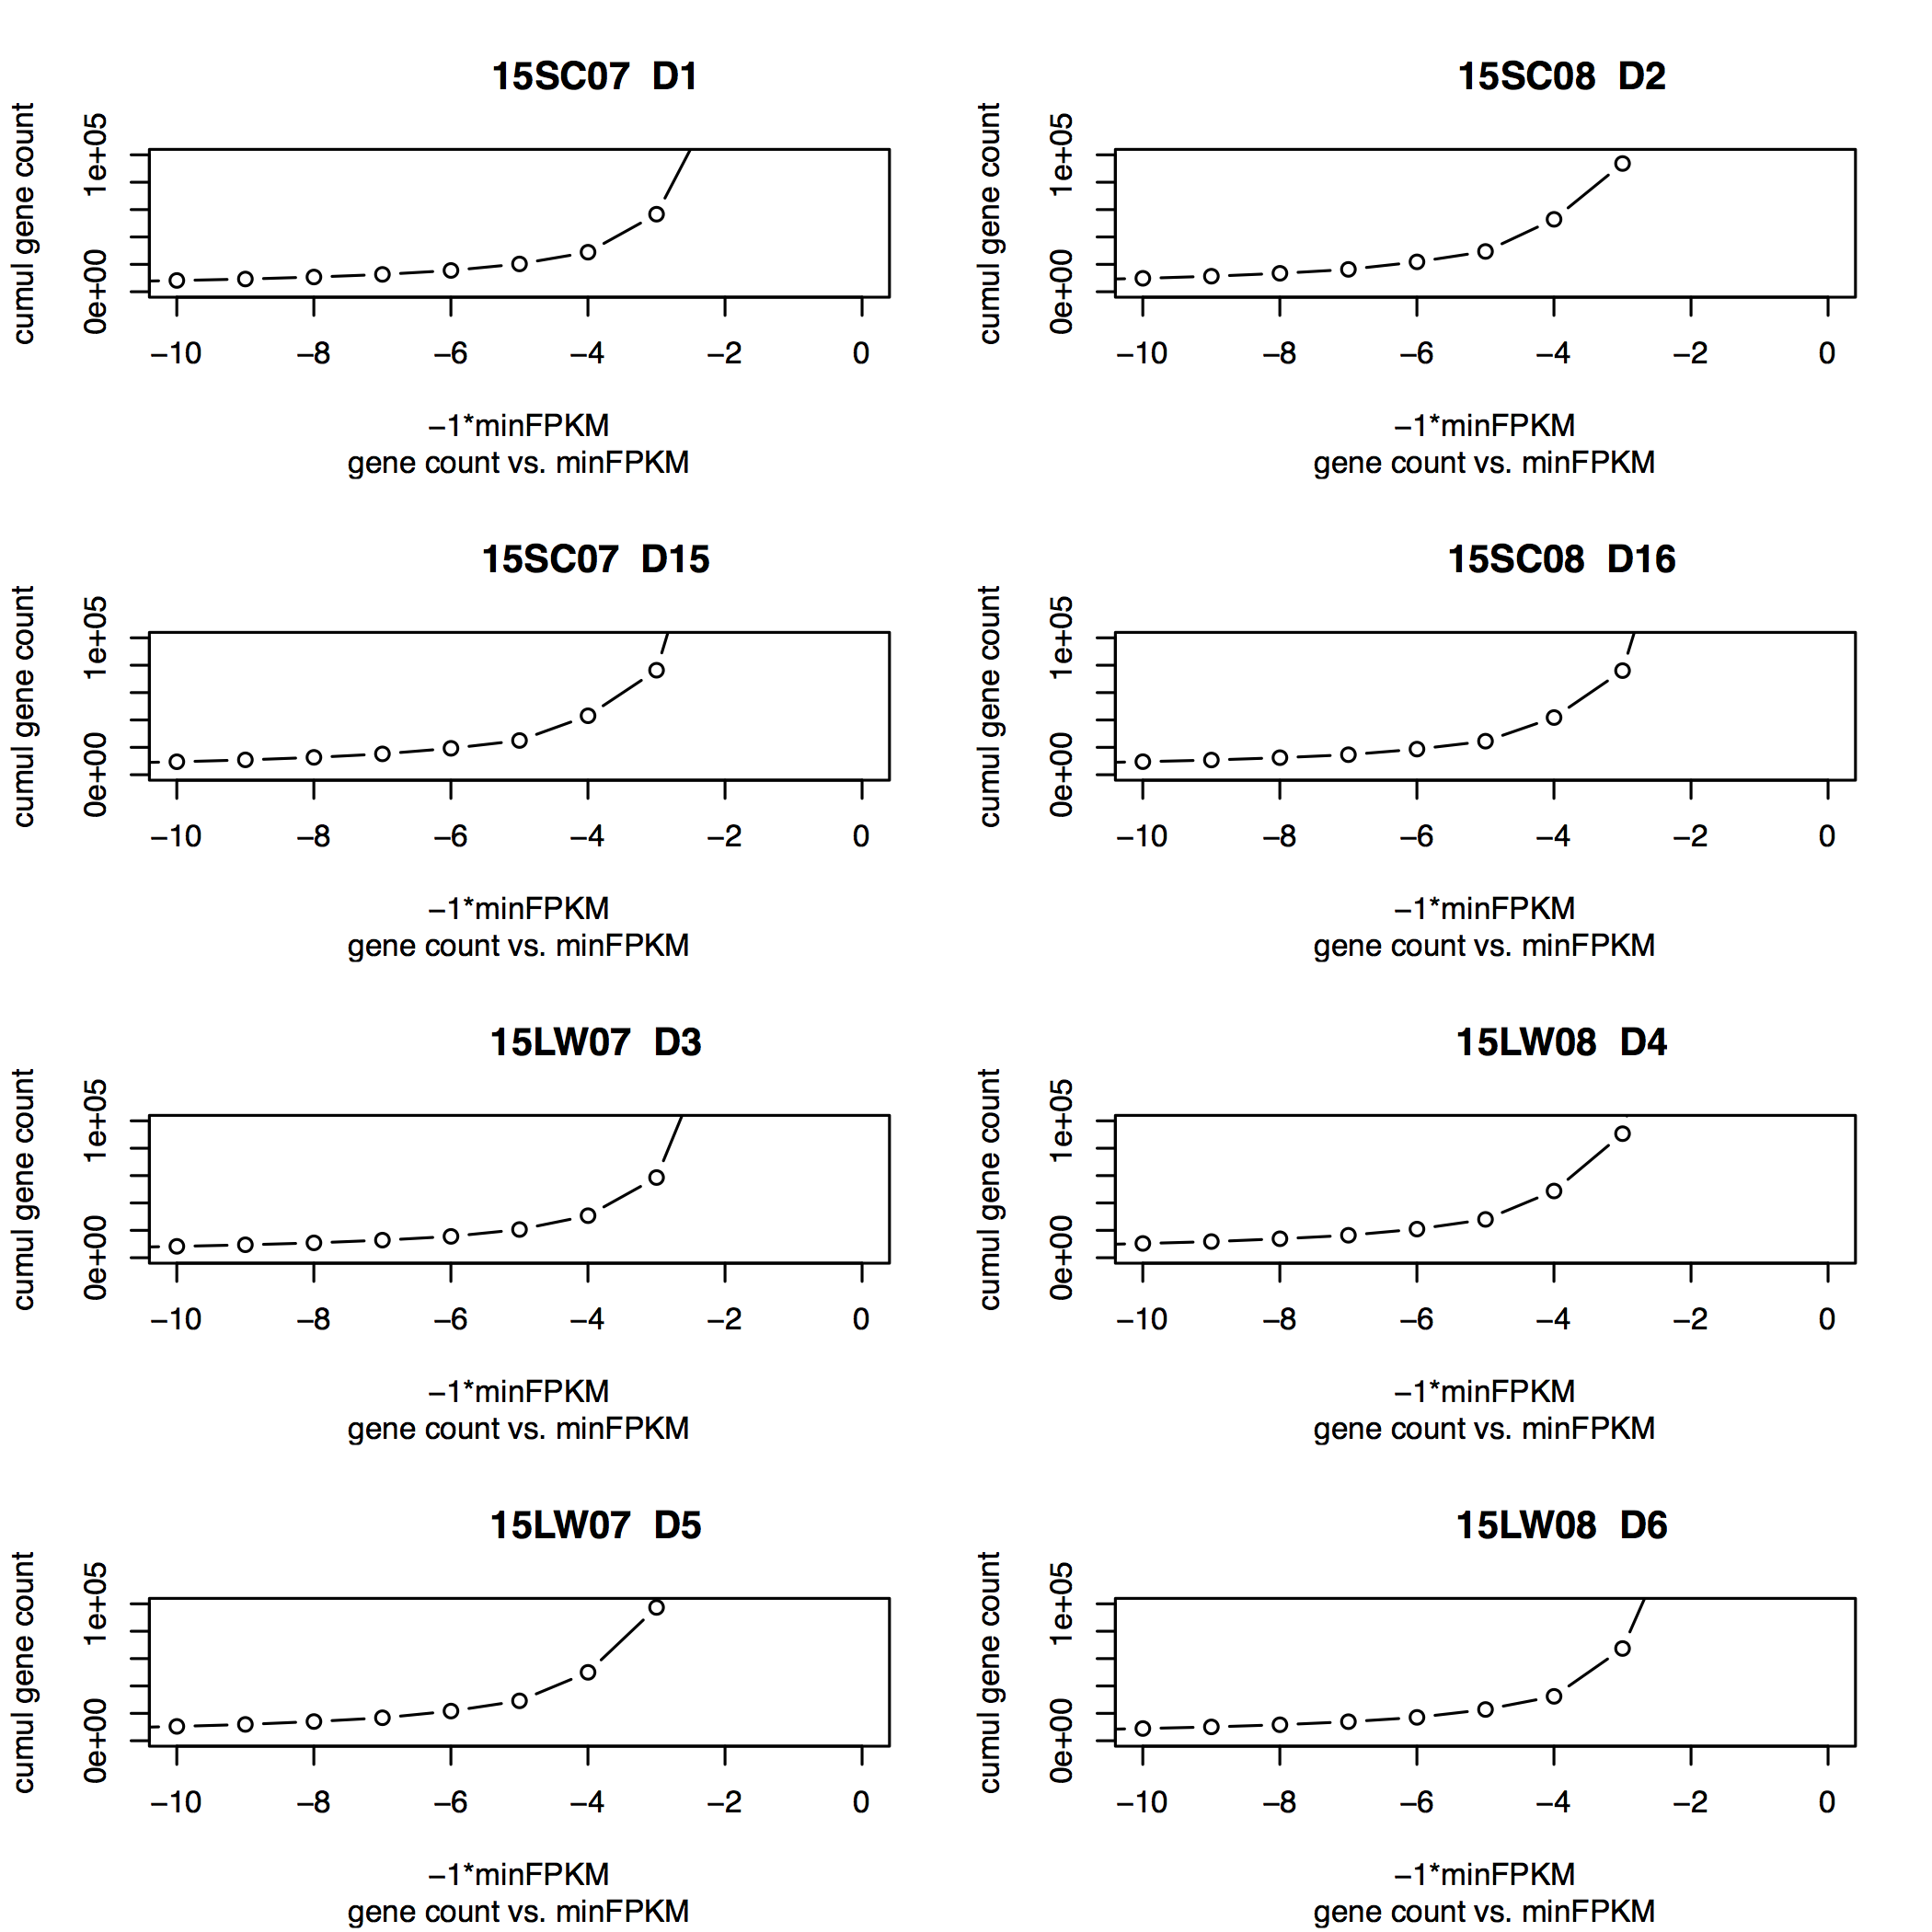
\includegraphics[width=\textwidth]{figs/fpkm.png}
    \caption{Cumulative transcript count (0 to 50,000) for several values of FPKM (0 to -10).}
    \label{fig:fpkm}
\end{figure}

\subsection{Differential expression}

Before TMM normalization, the number of DE transcripts identified with FDR of at most 0.05, 0.01, 0.005, and 0.001 are 2,469, 1,618, 1,404, and 1,129, respectively (see MA and Volcano plots in Figure~\ref{fig:plots}). After TMM normalization, the number of DE transcripts identified at FDR of 0.001 and fold change set at 4-fold if 1,114 (see transcript heat map in Figure~\ref{fig:heat}). By setting clusters of transcripts with similar expression profiles with the threshold at 60\% of transcript cluster dendrogram height, we found two distinct subclusters associated with low TTX or high TTX toxicity, as depicted in Figure~\ref{fig:clusters}. A total of 465 transcripts in subcluster 1 are more expressed in hight TTX toxicity condition. Subcluster 2 has 649 transcripts that are more expressed in low toxicity conditions.

\begin{figure}
    \centering
    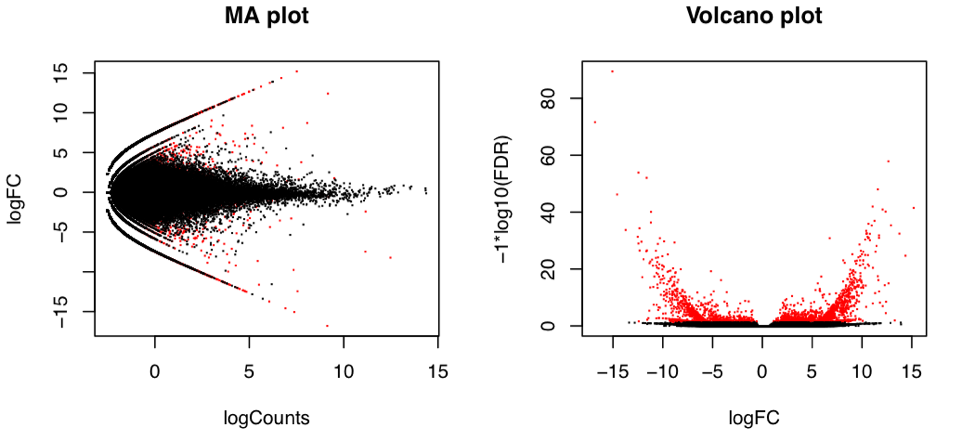
\includegraphics[width=\textwidth]{figs/plots.png}
    \caption{MA and Volcano plots showing equally (in black) and differently (in red) expressed transcripts.}
    \label{fig:plots}
\end{figure}

\begin{figure}
    \centering
    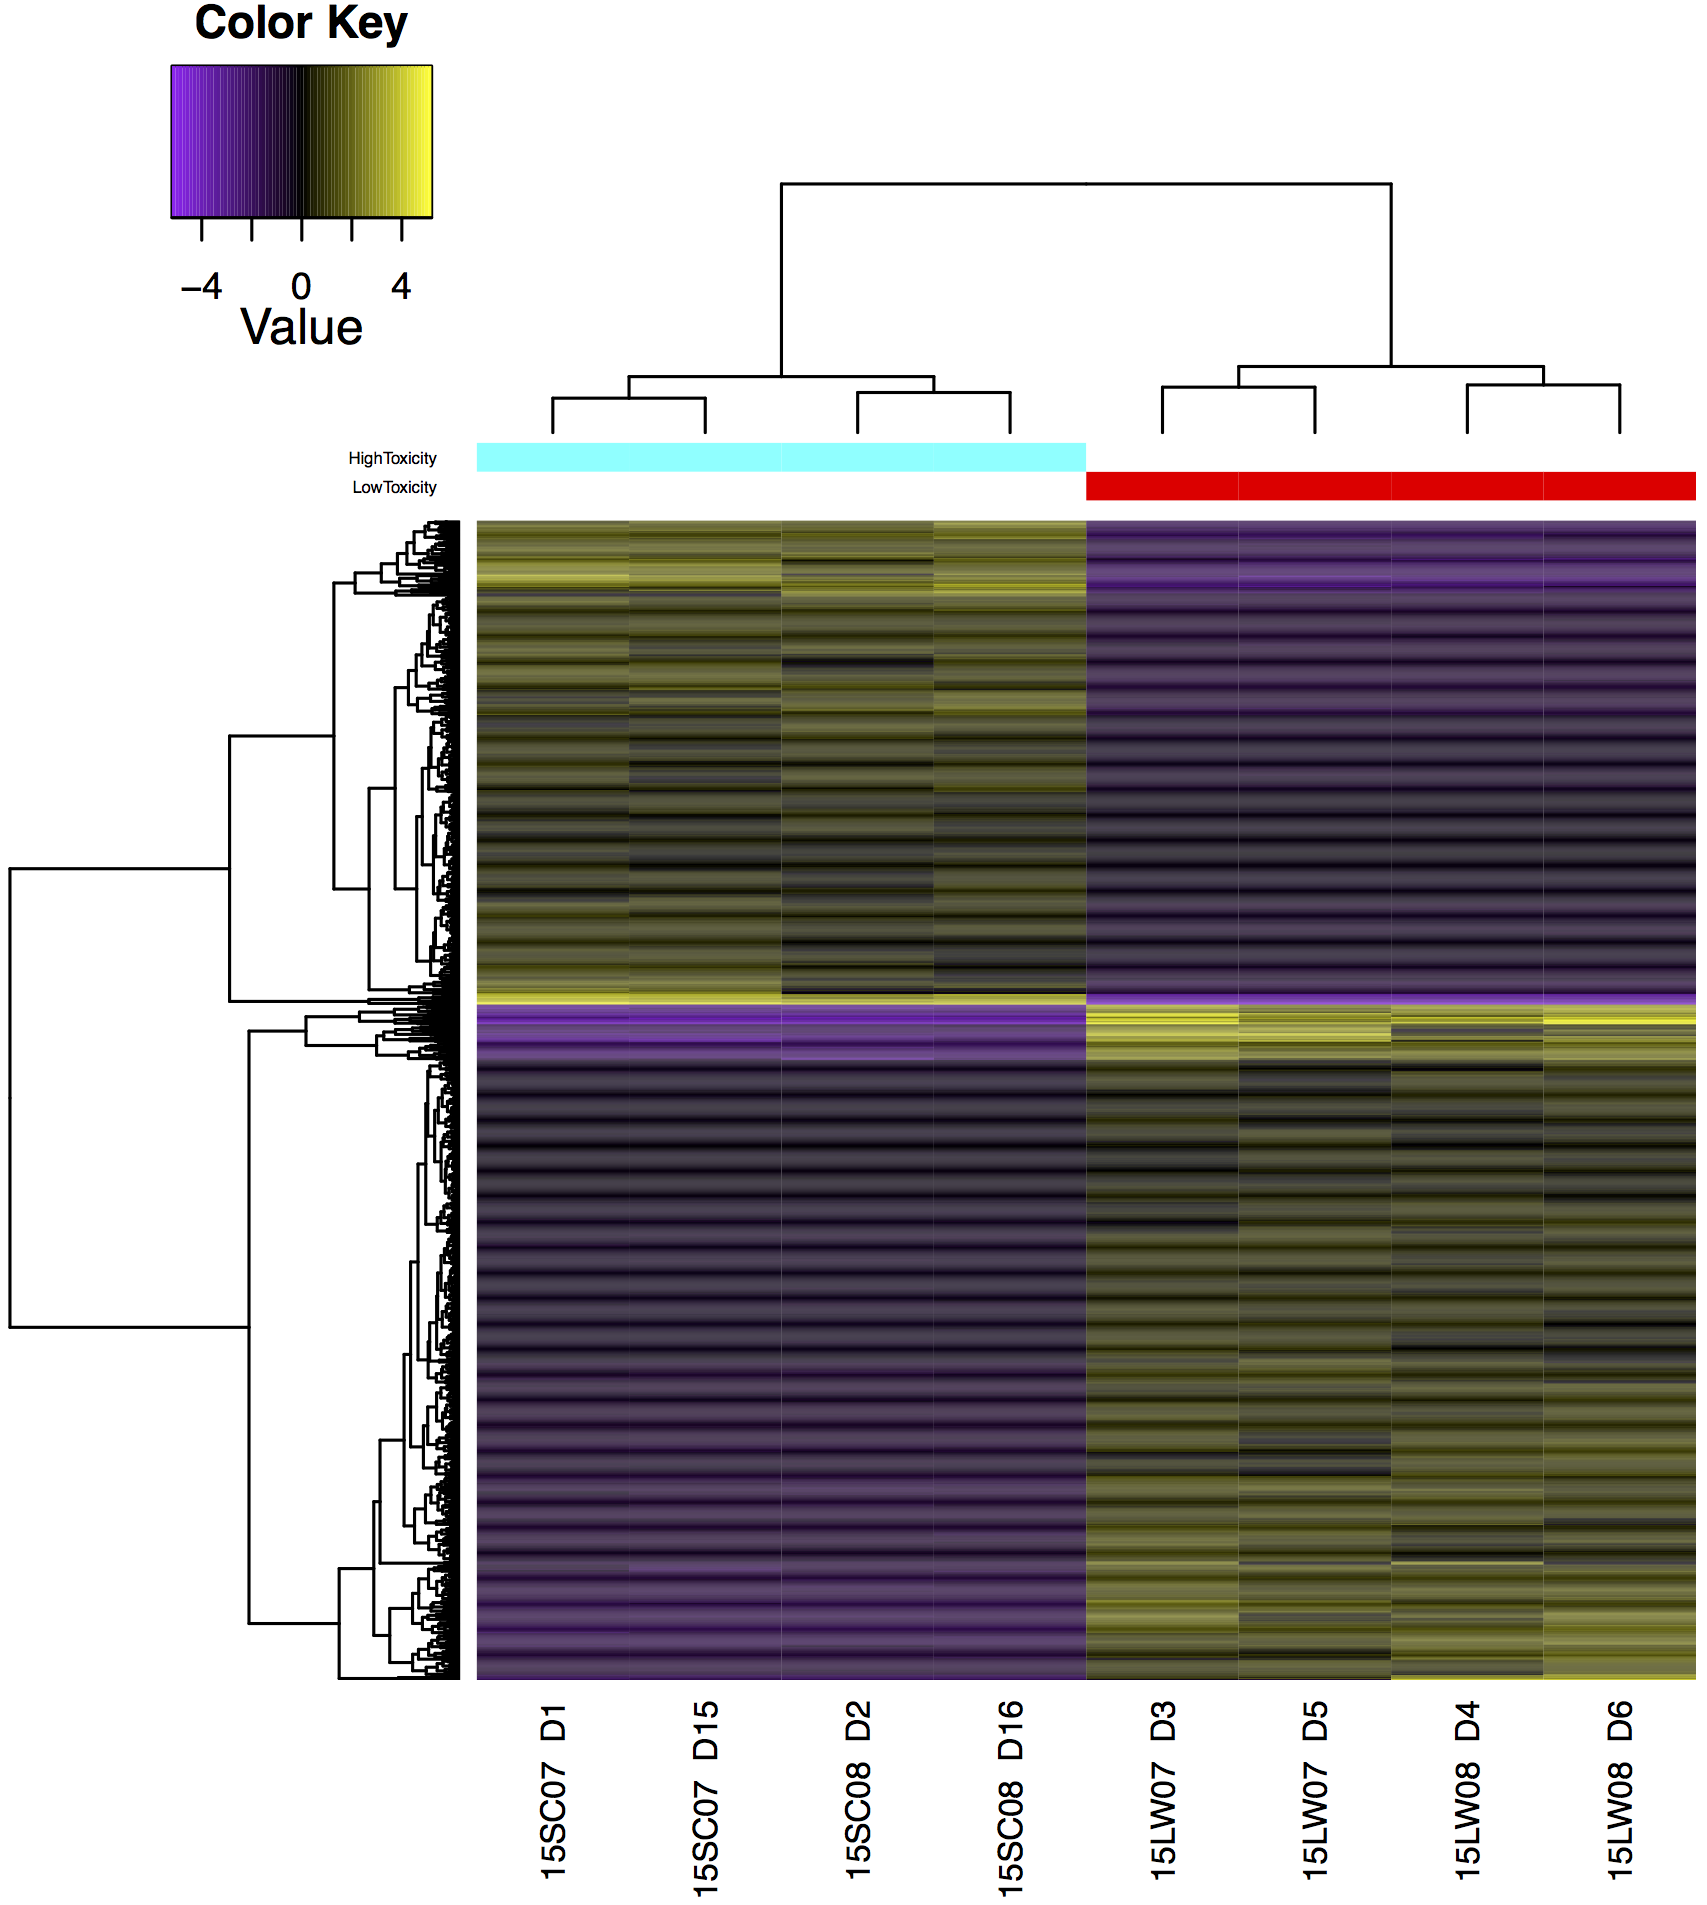
\includegraphics[width=\textwidth]{figs/heatmap.png}
    \caption{Heatmap showing transcripts clustered along the vertical axis and samples assembled along the horizontal axis.}
    \label{fig:heat}
\end{figure}

\begin{figure}
    \centering
    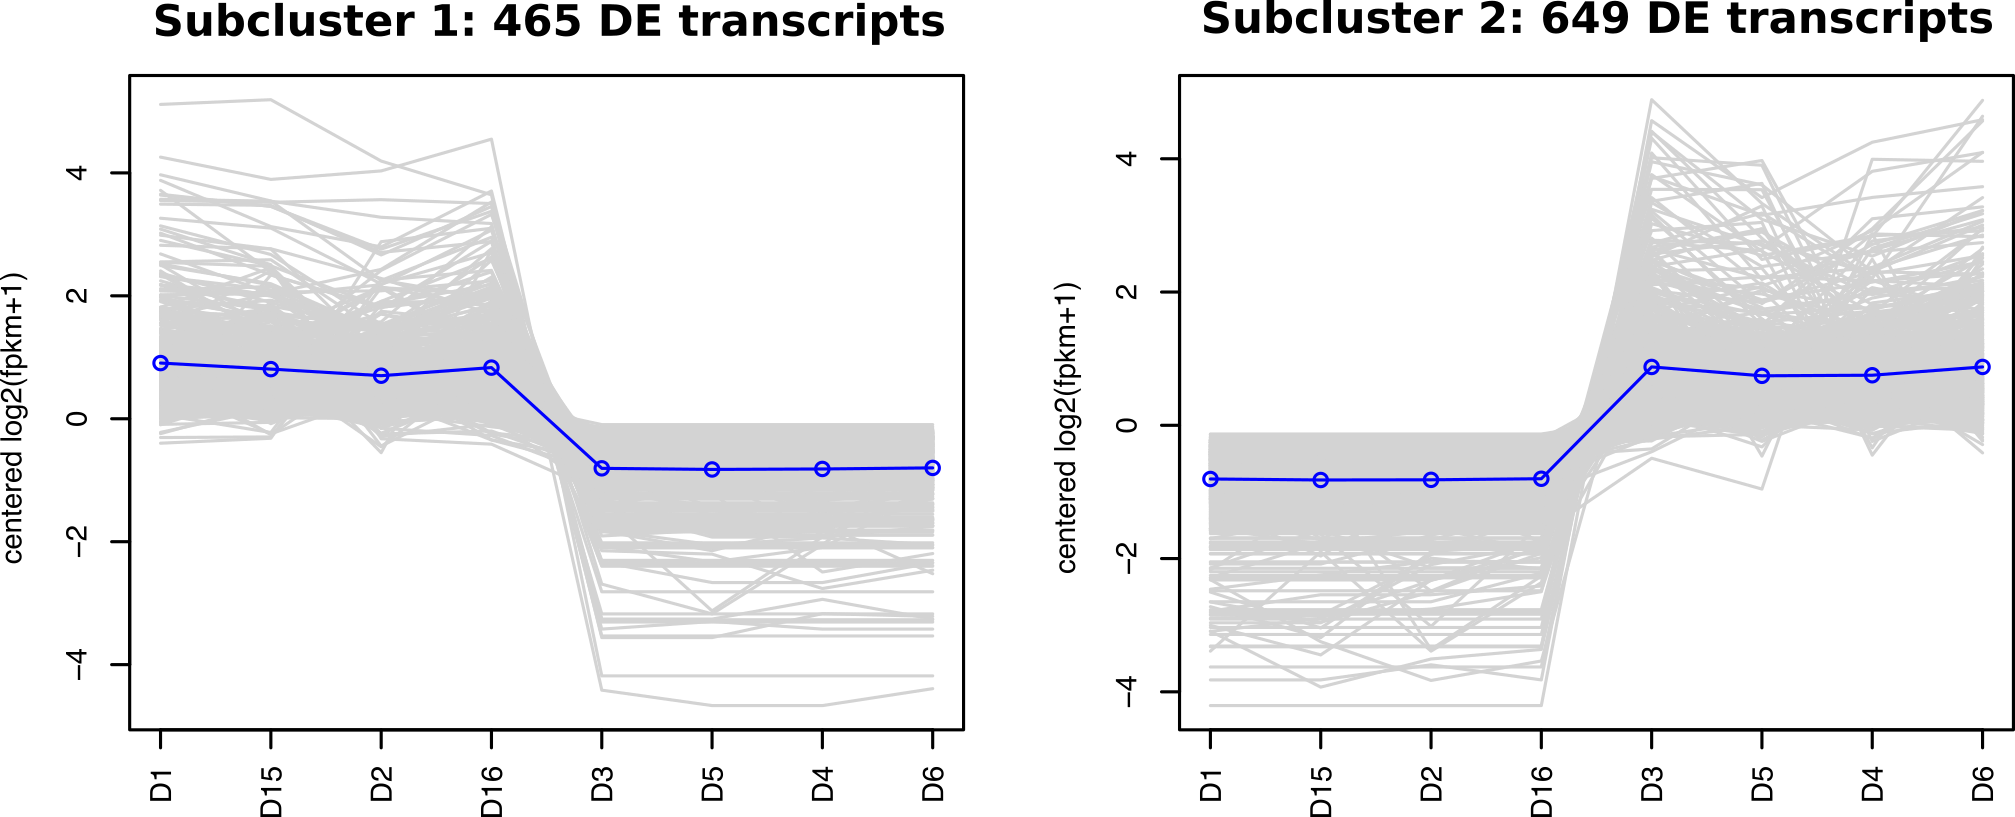
\includegraphics[width=\textwidth]{figs/clusters.png}
    \caption{Transcript clusters with similar expression profiles with the threshold at 60\% of transcript cluster dendrogram height. High toxicity biological replicates are on the left (D1, D2, D15, and D16) and low toxicity replicates are on the right (D3, D4, D5, and D6).}
    \label{fig:clusters}
\end{figure}

\subsection{Further data from amphibians}

As with \textit{Taricha granulosa}, we have begun analyzing \textit{Brachycephalus ephippium} transcriptomes in search of genes related to TTX. We assembled 229,391,603 RNA sequence reads from the skin of a specimen of Brachycephalus ephippium using Trinity v2.1.1 \citep{grabherr2011trinity} and following general guidelines provided by \citep{haas2013novo}. Trinity assembly resulted in 2,498,753 ``genes,'' with a total of 3,043,731 transcripts. We employed BUSCO v2 \citep{simao2015busco} to assess genome assembly and annotation completeness with single-copy orthologues of the Tetrapoda ODB9 database and found 3,159 of 3,950 (79.97\%) complete BUSCOs (42.63\% complete and single copy, 37.34\% complete and duplicates, 14\% fragmented, and 6.03\% missing). The assembled genes will be compared with our assemblies from \textit{T. granulosa} and published transcriptomes of other TTX-possessing / producing species to screen for possible gene similarities. We intend to produce another five transcriptomes of \textit{B. ephippium} and the non-TTX species \textit{B. hermogenesi} (totalizing 10 extra transcriptomes of \textit{Brachycephalus}).

\section{Research Expectations}

Samples from Soup Creek showed higher TTX toxicity levels (2127.100773 and 2520.537973 ng/mL) than samples from Lake in the Woods (-0.405706841 and 0.442922121 ng/mL). The sequencing we perfomed using using TruSeq ``total RNA'' library preparation kits with Ribo-Zero Gold and Illumina HiSeq 2500  with 125 bp paired-end reads yielded 747,043 to 1,175,336 sequences per sample. Preliminary analysis using BUSCO suggests that we sequenced 28–44\% of the single-copy orthologs of animals, a high percentage given that we targeted a single tissue type.

To date, I have identified 1,653 transcripts in the \textit{T}. \textit{granulosa} transcriptome that are more similar to sequences in other animals with TTX (especially on the tetraodon pufferfish) than to any other animal in the available databases. To complete this study, I propose to obtain an additional 10 \textit{T}. \textit{granulosa} transcriptomes. Candidate transcripts will be annotated and subjected to ontology analysis to identify the names and functions of differentially expressed genes. Sequences with little similarities to public databases will be flagged as potential new sequences, possibly underlying the metabolic pathway of TTX production.

As a strategy to optimize our search for TTX-related genes, we will compare candidate genes from the comparative transcriptome analysis of the rough-skinned newt with available transcriptomes of other TTX-possessing species. If we are capable of identifying strong gene candidates for TTX chemical defense, future research might take advantages of innovative techniques such as CRISPR (Cong et al., 2013) to perform functional tests.
